% Kommentare für den Editor (TexWorks/TexMakerX)
% !TeX encoding   = utf8
% !TeX spellcheck = de-DE

% Dokumentenklasse (Koma Script) -----------------------------------------
\documentclass[%
   %draft,     % Entwurfsstadium
   final,      % fertiges Dokument
   paper=a4, paper=portrait, pagesize=auto, % Papier Einstellungen
   fontsize=12pt, % Schriftgröße
   ngerman, % Sprache 
 ]{scrartcl} % Classes: scrartcl, scrreprt, scrbook

% ~~~~~~~~~~~~~~~~~~~~~~~~~~~~~~~~~~~~~~~~~~~~~~~~~~~~~~~~~~~~~~~~~~~~~~~~
% encoding
% ~~~~~~~~~~~~~~~~~~~~~~~~~~~~~~~~~~~~~~~~~~~~~~~~~~~~~~~~~~~~~~~~~~~~~~~~

% Encoding der Dateien (sonst funktionieren Umlaute nicht)
\usepackage[utf8]{inputenc}

% Encoding der Verzeichnisse (für Pfade mit Umlauten und Leerzeichne)
\usepackage[%
   extendedchars, encoding, multidot, space,
   filenameencoding=latin1, % Windows XP, Vista, 7
   % filenameencoding=utf8,   % Linux, OS X
]{grffile}

% ~~~~~~~~~~~~~~~~~~~~~~~~~~~~~~~~~~~~~~~~~~~~~~~~~~~~~~~~~~~~~~~~~~~~~~~~
% Pakete und Stile
% ~~~~~~~~~~~~~~~~~~~~~~~~~~~~~~~~~~~~~~~~~~~~~~~~~~~~~~~~~~~~~~~~~~~~~~~~
% Schriften
% ~~~~~~~~~~~~~~~~~~~~~~~~~~~~~~~~~~~~~~~~~~~~~~~~~~~~~~~~~~~~~~~~~~~~~~~~
% Fonts Fonts Fonts
% ~~~~~~~~~~~~~~~~~~~~~~~~~~~~~~~~~~~~~~~~~~~~~~~~~~~~~~~~~~~~~~~~~~~~~~~~

% immer laden:
\usepackage[T1]{fontenc} % T1 Schrift Encoding
\usepackage{textcomp}	 % Zusätzliche Symbole (Text Companion font extension)

% ~~~~~~~~~~~~~~~~~~~~~~~~~~~~~~~~~~~~~~~~~~~~~~~~~~~~~~~~~~~~~~~~~~~~~~~~
% Symbole
% ~~~~~~~~~~~~~~~~~~~~~~~~~~~~~~~~~~~~~~~~~~~~~~~~~~~~~~~~~~~~~~~~~~~~~~~~

\usepackage{amssymb}
\usepackage{mathcomp}


%% ==== Zusammengesetzte Schriften  (Sans + Serif) =======================

%% - Latin Modern
\usepackage{lmodern}
%% -------------------

%% - Bera Schriften
%\usepackage{bera}
%% -------------------

%% - Times, Helvetica, Courier (Word Standard...)
%\usepackage{mathptmx}
%\usepackage[scaled=.90]{helvet}
%\usepackage{courier}
%% -------------------

%% - Palantino , Helvetica, Courier
%\usepackage{mathpazo}
%\usepackage[scaled=.95]{helvet}
%\usepackage{courier}
%% -------------------

%% - Charter, Bera Sans
%\usepackage{charter}\linespread{1.05}
%\renewcommand{\sfdefault}{fvs}
%\usepackage[charter]{mathdesign}



%%%% =========== Typewriter =============

%\usepackage{courier}                   %% --- Courier
%\renewcommand{\ttdefault}{cmtl}        %% --- CmBright Typewriter Font
%\usepackage[%                          %% --- Luxi Mono (Typewriter)
%   scaled=0.9
%]{luximono}



% Pakete Laden
% ~~~~~~~~~~~~~~~~~~~~~~~~~~~~~~~~~~~~~~~~~~~~~~~~~~~~~~~~~~~~~~~~~~~~~~~~
% These packages must be loaded before all others
% (primarily because they are required by other packages)
% ~~~~~~~~~~~~~~~~~~~~~~~~~~~~~~~~~~~~~~~~~~~~~~~~~~~~~~~~~~~~~~~~~~~~~~~~
\usepackage{calc}
\usepackage{fixltx2e}	% Fix known LaTeX2e bugs

\usepackage[ngerman]{babel} 			% Sprache
\usepackage[dvipsnames, table]{xcolor} 	% Farben

% ~~~~~~~~~~~~~~~~~~~~~~~~~~~~~~~~~~~~~~~~~~~~~~~~~~~~~~~~~~~~~~~~~~~~~~~~
% Bilder, Gleitumgebungen und Platzierung
% ~~~~~~~~~~~~~~~~~~~~~~~~~~~~~~~~~~~~~~~~~~~~~~~~~~~~~~~~~~~~~~~~~~~~~~~~

\usepackage[]{graphicx}					% Graphiken
\usepackage{epstopdf}		% konvertiert eps in pdf

% provides new floats and enables H float modifier option
\usepackage{float}
% Floats immer erst nach der Referenz setzen
\usepackage{flafter}
% Alel Floats werden vor der nächsten section ausgegeben
\usepackage[section]{placeins} 
%

% ~~~~~~~~~~~~~~~~~~~~~~~~~~~~~~~~~~~~~~~~~~~~~~~~~~~~~~~~~~~~~~~~~~~~~~~~
% Beschriftungen (captions)
% ~~~~~~~~~~~~~~~~~~~~~~~~~~~~~~~~~~~~~~~~~~~~~~~~~~~~~~~~~~~~~~~~~~~~~~~~

\usepackage{caption}
\usepackage{subcaption}

% ~~~~~~~~~~~~~~~~~~~~~~~~~~~~~~~~~~~~~~~~~~~~~~~~~~~~~~~~~~~~~~~~~~~~~~~~
% Math
% ~~~~~~~~~~~~~~~~~~~~~~~~~~~~~~~~~~~~~~~~~~~~~~~~~~~~~~~~~~~~~~~~~~~~~~~~

% Base Math Package
\usepackage[fleqn]{amsmath} 
% Warnt bei Benutzung von Befehlen die mit amsmath inkompatibel sind.
\usepackage[all, error]{onlyamsmath}

% ~~~~~~~~~~~~~~~~~~~~~~~~~~~~~~~~~~~~~~~~~~~~~~~~~~~~~~~~~~~~~~~~~~~~~~~~
% Science
% ~~~~~~~~~~~~~~~~~~~~~~~~~~~~~~~~~~~~~~~~~~~~~~~~~~~~~~~~~~~~~~~~~~~~~~~~

% Einheiten und Zahlenformatierung
\usepackage{siunitx}

% ~~~~~~~~~~~~~~~~~~~~~~~~~~~~~~~~~~~~~~~~~~~~~~~~~~~~~~~~~~~~~~~~~~~~~~~~
% Tables (Tabular)
% ~~~~~~~~~~~~~~~~~~~~~~~~~~~~~~~~~~~~~~~~~~~~~~~~~~~~~~~~~~~~~~~~~~~~~~~~

\usepackage{booktabs}
\usepackage{ltxtable} % Longtable + tabularx
\usepackage{threeparttable}

% ~~~~~~~~~~~~~~~~~~~~~~~~~~~~~~~~~~~~~~~~~~~~~~~~~~~~~~~~~~~~~~~~~~~~~~~~
% text related packages
% ~~~~~~~~~~~~~~~~~~~~~~~~~~~~~~~~~~~~~~~~~~~~~~~~~~~~~~~~~~~~~~~~~~~~~~~~

\usepackage{url}            % Befehl \url{...}
\usepackage{enumitem}		% Kompakte Listen

% Neue Befehle: \Centering, \RaggedLeft, and \RaggedRight, ... 
\usepackage{ragged2e}

\usepackage{listings}
\lstset{language=bash}
\usepackage{color}

% ~~~~~~~~~~~~~~~~~~~~~~~~~~~~~~~~~~~~~~~~~~~~~~~~~~~~~~~~~~~~~~~~~~~~~~~~
% Citations
% ~~~~~~~~~~~~~~~~~~~~~~~~~~~~~~~~~~~~~~~~~~~~~~~~~~~~~~~~~~~~~~~~~~~~~~~~

%\usepackage[
%	style=alphabetic, % Loads the bibliography and the citation style 
%	natbib=true, % define natbib compatible cite commands
%]{biblatex}	
% Other options:
%	style=numeric, % 
%	style=numeric-comp,    % [1–3, 7, 8]
%	style=numeric-verb,    % [2]; [5]; [6]


% ~~~~~~~~~~~~~~~~~~~~~~~~~~~~~~~~~~~~~~~~~~~~~~~~~~~~~~~~~~~~~~~~~~~~~~~~
% layout packages
% ~~~~~~~~~~~~~~~~~~~~~~~~~~~~~~~~~~~~~~~~~~~~~~~~~~~~~~~~~~~~~~~~~~~~~~~~
%
% Befehle für 1,5 und 2 zeilig: 
% \singlespacing, \onehalfspacing und \doublespacing
\usepackage{setspace}

% ~~~~~~~~~~~~~~~~~~~~~~~~~~~~~~~~~~~~~~~~~~~~~~~~~~~~~~~~~~~~~~~~~~~~~~~~
% Kopf und Fusszeile
% ~~~~~~~~~~~~~~~~~~~~~~~~~~~~~~~~~~~~~~~~~~~~~~~~~~~~~~~~~~~~~~~~~~~~~~~~

% Kopf und Fusszeile mit scrpage2 einstellen
\usepackage[automark, komastyle, nouppercase]{scrpage2}

% ~~~~~~~~~~~~~~~~~~~~~~~~~~~~~~~~~~~~~~~~~~~~~~~~~~~~~~~~~~~~~~~~~~~~~~~~
% pdf packages
% ~~~~~~~~~~~~~~~~~~~~~~~~~~~~~~~~~~~~~~~~~~~~~~~~~~~~~~~~~~~~~~~~~~~~~~~~

% Include pages from external PDF documents in LaTeX documents
\usepackage{pdfpages} 

% Optischer Randausgleich mit pdfTeX
\usepackage{microtype}

\usepackage[unicode]{hyperref}

\usepackage{listings}
% Einstellungen und Layoutstile 
% ~~~~~~~~~~~~~~~~~~~~~~~~~~~~~~~~~~~~~~~~~~~~~~~~~~~~~~~~~~~~~~~~~~~~~~~~
% Colors
% ~~~~~~~~~~~~~~~~~~~~~~~~~~~~~~~~~~~~~~~~~~~~~~~~~~~~~~~~~~~~~~~~~~~~~~~~
\definecolor{sectioncolor}{RGB}{0, 0, 0}     % black

% ~~~~~~~~~~~~~~~~~~~~~~~~~~~~~~~~~~~~~~~~~~~~~~~~~~~~~~~~~~~~~~~~~~~~~~~~
% text related 
% ~~~~~~~~~~~~~~~~~~~~~~~~~~~~~~~~~~~~~~~~~~~~~~~~~~~~~~~~~~~~~~~~~~~~~~~~

%% style of URL
\urlstyle{tt}


% Keine hochgestellten Ziffern in der Fussnote (KOMA-Script-spezifisch):
\deffootnote{1.5em}{1em}{\makebox[1.5em][l]{\thefootnotemark}}

% Limit space of footnotes to 10 lines
\setlength{\dimen\footins}{10\baselineskip}

% prevent continuation of footnotes 
% at facing page
\interfootnotelinepenalty=10000 

% ~~~~~~~~~~~~~~~~~~~~~~~~~~~~~~~~~~~~~~~~~~~~~~~~~~~~~~~~~~~~~~~~~~~~~~~~
% Science
% ~~~~~~~~~~~~~~~~~~~~~~~~~~~~~~~~~~~~~~~~~~~~~~~~~~~~~~~~~~~~~~~~~~~~~~~~

\sisetup{%
	mode = math, detect-family, detect-weight,	
	exponent-product = \cdot,
	number-unit-separator=\text{\,},
	output-decimal-marker={,},
}

% ~~~~~~~~~~~~~~~~~~~~~~~~~~~~~~~~~~~~~~~~~~~~~~~~~~~~~~~~~~~~~~~~~~~~~~~~
% Citations / Style of Bibliography
% ~~~~~~~~~~~~~~~~~~~~~~~~~~~~~~~~~~~~~~~~~~~~~~~~~~~~~~~~~~~~~~~~~~~~~~~~

% Kommentar entfernene wenn biblatex geladen wird
% \IfPackageLoaded{biblatex}{%
	\ExecuteBibliographyOptions{%
%--- Backend --- --- ---
	backend=bibtex,  % (bibtex, bibtex8, biber)
	bibwarn=true, %
	bibencoding=ascii, % (ascii, inputenc, <encoding>)
%--- Sorting --- --- ---
	sorting=nty, % Sort by name, title, year.
	% other options: 
	% nty        Sort by name, title, year.
	% nyt        Sort by name, year, title.
	% nyvt       Sort by name, year, volume, title.
	% anyt       Sort by alphabetic label, name, year, title.
	% anyvt      Sort by alphabetic label, name, year, volume, title.
	% ynt        Sort by year, name, title.
	% ydnt       Sort by year (descending), name, title.
	% none       Do not sort at all. All entries are processed in citation order.
	% debug      Sort by entry key. This is intended for debugging only.
	%
	sortcase=true,
	sortlos=los, % (bib, los) The sorting order of the list of shorthands
	sortcites=false, % do/do not sort citations according to bib	
%--- Dates --- --- ---
	date=comp,  % (short, long, terse, comp, iso8601)
%	origdate=
%	eventdate=
%	urldate=
%	alldates=
	datezeros=true, %
	dateabbrev=true, %
%--- General Options --- --- ---
	maxnames=1,
	minnames=1,
%	maxbibnames=99,
%	maxcitenames=1,
%	autocite= % (plain, inline, footnote, superscript) 
	autopunct=true,
	language=auto,
	babel=none, % (none, hyphen, other, other*)
	block=none, % (none, space, par, nbpar, ragged)
	notetype=foot+end, % (foot+end, footonly, endonly)
	hyperref=true, % (true, false, auto)
	backref=true,
	backrefstyle=three, % (none, three, two, two+, three+, all+)
	backrefsetstyle=setonly, %
	indexing=false, % 
	% options:
	% true       Enable indexing globally.
	% false      Disable indexing globally.
	% cite       Enable indexing in citations only.
	% bib        Enable indexing in the bibliography only.
	refsection=none, % (part, chapter, section, subsection)
	refsegment=none, % (none, part, chapter, section, subsection)
	abbreviate=true, % (true, false)
	defernumbers=false, % 
	punctfont=false, % 
	arxiv=abs, % (ps, pdf, format)	
%--- Style Options --- --- ---	
% The following options are provided by the standard styles
	isbn=false,%
	url=false,%
	doi=false,%
	eprint=false,%	
	}%	
	
	% change alpha label to be without +	
	\renewcommand*{\labelalphaothers}{}
	
	% change 'In: <magazine>" to "<magazine>"
	\renewcommand*{\intitlepunct}{}
	\DefineBibliographyStrings{german}{in={}}
	
	% make names capitalized \textsc{}
	\renewcommand{\mkbibnamefirst}{\textsc}
	\renewcommand{\mkbibnamelast}{\textsc}
	
	% make volume and number look like 
	% 'Bd. 33(14): '
	\renewbibmacro*{volume+number+eid}{%
	  \setunit{\addcomma\space}%
	  \bibstring{volume}% 
	  \setunit{\addspace}%
	  \printfield{volume}%
	  \iffieldundef{number}{}{% 
	    \printtext[parens]{%
	      \printfield{number}%
	    }%
	  }%
	  \setunit{\addcomma\space}%
	  \printfield{eid}
	  %\setunit{\addcolon\space}%
	  }	

	% <authors>: <title>
	\renewcommand*{\labelnamepunct}{\addcolon\space}
	% make ': ' before pages
	\renewcommand*{\bibpagespunct}{\addcolon\space}
	% names delimiter ';' instead of ','
	%\renewcommand*{\multinamedelim}{\addsemicolon\space}

	% move date before issue
	\renewbibmacro*{journal+issuetitle}{%
	  \usebibmacro{journal}%
	  \setunit*{\addspace}%
	  \iffieldundef{series}
	    {}
	    {\newunit
	     \printfield{series}%
	     \setunit{\addspace}}%
	  %
	  \usebibmacro{issue+date}%
	  \setunit{\addcolon\space}%
	  \usebibmacro{issue}%
	  \setunit{\addspace}%
	  \usebibmacro{volume+number+eid}%
	  \newunit}

	% print all names, even if maxnames = 1
	\DeclareCiteCommand{\citeauthors}
	  {
	   \defcounter{maxnames}{1000}
	   \boolfalse{citetracker}%
	   \boolfalse{pagetracker}%
	   \usebibmacro{prenote}}
	  {\ifciteindex
	     {\indexnames{labelname}}
	     {}%
	   \printnames{labelname}}
	  {\multicitedelim}
	  {\usebibmacro{postnote}}

}%

% ~~~~~~~~~~~~~~~~~~~~~~~~~~~~~~~~~~~~~~~~~~~~~~~~~~~~~~~~~~~~~~~~~~~~~~~~
% figures, placement, floats and captions
% ~~~~~~~~~~~~~~~~~~~~~~~~~~~~~~~~~~~~~~~~~~~~~~~~~~~~~~~~~~~~~~~~~~~~~~~~

% Make float placement easier
\renewcommand{\floatpagefraction}{.75} % vorher: .5
\renewcommand{\textfraction}{.1}       % vorher: .2
\renewcommand{\topfraction}{.8}        % vorher: .7
\renewcommand{\bottomfraction}{.5}     % vorher: .3
\setcounter{topnumber}{3}        % vorher: 2
\setcounter{bottomnumber}{2}     % vorher: 1
\setcounter{totalnumber}{5}      % vorher: 3

%% ~~~ Captions ~~~~~~~~~~~~~~~~~~~~~~~~~~~~~~~~~~~~~~~~~~~~~~~~~~~~~~~~~~
% Style of captions
\DeclareCaptionStyle{captionStyleTemplateDefault}
[ % single line captions
   justification = centering
]
{ % multiline captions
% -- Formatting
   format      = plain,  % plain, hang
   indention   = 0em,    % indention of text 
   labelformat = default,% default, empty, simple, brace, parens
   labelsep    = colon,  % none, colon, period, space, quad, newline, endash
   textformat  = simple, % simple, period
% -- Justification
   justification = justified, %RaggedRight, justified, centering
   singlelinecheck = true, % false (true=ignore justification setting in single line)
% -- Fonts
   labelfont   = {small,bf},
   textfont    = {small,rm},
% valid values:
% scriptsize, footnotesize, small, normalsize, large, Large
% normalfont, ip, it, sl, sc, md, bf, rm, sf, tt
% singlespacing, onehalfspacing, doublespacing
% normalcolor, color=<...>
%
% -- Margins and further paragraph options
   margin = 10pt, %.1\textwidth,
   % width=.8\linewidth,
% -- Skips
   skip     = 10pt, % vertical space between the caption and the figure
   position = auto, % top, auto, bottom
% -- Lists
   % list=no, % suppress any entry to list of figure 
   listformat = subsimple, % empty, simple, parens, subsimple, subparens
% -- Names & Numbering
   % figurename = Abb. %
   % tablename  = Tab. %
   % listfigurename=
   % listtablename=
   % figurewithin=chapter
   % tablewithin=chapter
%-- hyperref related options
	hypcap=true, % (true, false) 
	% true=all hyperlink anchors are placed at the 
	% beginning of the (floating) environment
	%
	hypcapspace=0.5\baselineskip
}

% apply caption style
\captionsetup{
	style = captionStyleTemplateDefault % base
}

% Predefinded skip setup for different floats
\captionsetup[table]{position=top}
\captionsetup[figure]{position=bottom}


% options for subcaptions
\captionsetup[sub]{ %
	style = captionStyleTemplateDefault, % base
	skip=6pt,
	margin=5pt,
	labelformat = parens,% default, empty, simple, brace
	labelsep    = space,
	list=false,
	hypcap=false
}

% ~~~~~~~~~~~~~~~~~~~~~~~~~~~~~~~~~~~~~~~~~~~~~~~~~~~~~~~~~~~~~~~~~~~~~~~~
% layout 
% ~~~~~~~~~~~~~~~~~~~~~~~~~~~~~~~~~~~~~~~~~~~~~~~~~~~~~~~~~~~~~~~~~~~~~~~~


%% Paragraph Separation =================================
\KOMAoptions{%
   parskip=absolute, % do not change indentation according to fontsize
   parskip=false     % indentation of 1em
   % parskip=half    % parksip of 1/2 line 
}%

%% line spacing =========================================
%\onehalfspacing	% 1,5-facher Abstand
%\doublespacing		% 2-facher Abstand

%% page layout ==========================================

\raggedbottom     % Variable Seitenhoehen zulassen

% Koma Script text area layout
\KOMAoptions{%
   DIV=11,% (Size of Text Body, higher values = greater textbody)
   BCOR=5mm% (Bindekorrektur)
}%

%%% === Page Layout  Options ===
\KOMAoptions{% (most options are for package typearea)
   % twoside=true, % two side layout (alternating margins, standard in books)
   twoside=false, % single side layout 
   %
   headlines=2.1,%
}%

%\KOMAoptions{%
%      headings=noappendixprefix % chapter in appendix as in body text
%      ,headings=nochapterprefix  % no prefix at chapters
%      % ,headings=appendixprefix   % inverse of 'noappendixprefix'
%      % ,headings=chapterprefix    % inverse of 'nochapterprefix'
%      % ,headings=openany   % Chapters start at any side
%      % ,headings=openleft  % Chapters start at left side
%      ,headings=openright % Chapters start at right side      
%}%


% reloading of typearea, necessary if setting of spacing changed
\typearea[current]{last}

% ~~~~~~~~~~~~~~~~~~~~~~~~~~~~~~~~~~~~~~~~~~~~~~~~~~~~~~~~~~~~~~~~~~~~~~~~
% Titlepage
% ~~~~~~~~~~~~~~~~~~~~~~~~~~~~~~~~~~~~~~~~~~~~~~~~~~~~~~~~~~~~~~~~~~~~~~~~
\KOMAoptions{%
   % titlepage=true %
   titlepage=false %
}%

% ~~~~~~~~~~~~~~~~~~~~~~~~~~~~~~~~~~~~~~~~~~~~~~~~~~~~~~~~~~~~~~~~~~~~~~~~
% head and foot lines
% ~~~~~~~~~~~~~~~~~~~~~~~~~~~~~~~~~~~~~~~~~~~~~~~~~~~~~~~~~~~~~~~~~~~~~~~~

% \pagestyle{scrheadings} % Seite mit Headern
\pagestyle{scrplain} % Seiten ohne Header

% loescht voreingestellte Stile
\clearscrheadings
\clearscrplain
%
% Was steht wo...
% Bei headings:
%   % Oben aussen: Kapitel und Section
%   % Unten aussen: Seitenzahl
%   \ohead{\pagemark}
%   \ihead{\headmark}
%   \ofoot[\pagemark]{} % Außen unten: Seitenzahlen bei plain
% Bei Plain:
\cfoot[\pagemark]{\pagemark} % Mitte unten: Seitenzahlen bei plain


% Angezeigte Abschnitte im Header
% \automark[section]{chapter} %[rechts]{links}
\automark[subsection]{section} %[rechts]{links}

% ~~~~~~~~~~~~~~~~~~~~~~~~~~~~~~~~~~~~~~~~~~~~~~~~~~~~~~~~~~~~~~~~~~~~~~~~
% headings / page opening
% ~~~~~~~~~~~~~~~~~~~~~~~~~~~~~~~~~~~~~~~~~~~~~~~~~~~~~~~~~~~~~~~~~~~~~~~~
\setcounter{secnumdepth}{2}

\KOMAoptions{%
%%%% headings
   % headings=small  % Small Font Size, thin spacing above and below
   % headings=normal % Medium Font Size, medium spacing above and below
   headings=big % Big Font Size, large spacing above and below
}%

% Titelzeile linksbuendig, haengend
\renewcommand*{\raggedsection}{\raggedright} 

% ~~~~~~~~~~~~~~~~~~~~~~~~~~~~~~~~~~~~~~~~~~~~~~~~~~~~~~~~~~~~~~~~~~~~~~~~
% fonts of headings
% ~~~~~~~~~~~~~~~~~~~~~~~~~~~~~~~~~~~~~~~~~~~~~~~~~~~~~~~~~~~~~~~~~~~~~~~~
\setkomafont{sectioning}{\normalfont\sffamily} % \rmfamily
\setkomafont{descriptionlabel}{\itshape}
\setkomafont{pageheadfoot}{\normalfont\normalcolor\small\sffamily}
\setkomafont{pagenumber}{\normalfont\sffamily}

%%% --- Titlepage ---
%\setkomafont{subject}{}
%\setkomafont{subtitle}{}
%\setkomafont{title}{}

% ~~~~~~~~~~~~~~~~~~~~~~~~~~~~~~~~~~~~~~~~~~~~~~~~~~~~~~~~~~~~~~~~~~~~~~~~
% settings and layout of TOC, LOF, 
% ~~~~~~~~~~~~~~~~~~~~~~~~~~~~~~~~~~~~~~~~~~~~~~~~~~~~~~~~~~~~~~~~~~~~~~~~
\setcounter{tocdepth}{3} % Depth of TOC Display

% ~~~~~~~~~~~~~~~~~~~~~~~~~~~~~~~~~~~~~~~~~~~~~~~~~~~~~~~~~~~~~~~~~~~~~~~~
% Tabellen
% ~~~~~~~~~~~~~~~~~~~~~~~~~~~~~~~~~~~~~~~~~~~~~~~~~~~~~~~~~~~~~~~~~~~~~~~~

%%% -| Neue Spaltendefinitionen 'columntypes' |--
%
% Belegte Spaltentypen:
% l - links
% c - zentriert
% r - rechts
% p,m,b  - oben, mittig, unten
% X - tabularx Auto-Spalte

% um Tabellenspalten mit Flattersatz zu setzen, muss \\ vor
% (z.B.) \raggedright geschuetzt werden:
\newcommand{\PreserveBackslash}[1]{\let\temp=\\#1\let\\=\temp}

% Spalten mit Flattersatz und definierte Breite:
% m{} -> mittig
% p{} -> oben
% b{} -> unten
%
% Linksbuendig:
\newcolumntype{v}[1]{>{\PreserveBackslash\RaggedRight\hspace{0pt}}p{#1}}
\newcolumntype{M}[1]{>{\PreserveBackslash\RaggedRight\hspace{0pt}}m{#1}}
% % Rechtsbuendig :
% \newcolumntype{R}[1]{>{\PreserveBackslash\RaggedLeft\hspace{0pt}}m{#1}}
% \newcolumntype{S}[1]{>{\PreserveBackslash\RaggedLeft\hspace{0pt}}p{#1}}
% % Zentriert :
% \newcolumntype{Z}[1]{>{\PreserveBackslash\Centering\hspace{0pt}}m{#1}}
% \newcolumntype{A}[1]{>{\PreserveBackslash\Centering\hspace{0pt}}p{#1}}

\newcolumntype{Y}{>{\PreserveBackslash\RaggedLeft\hspace{0pt}}X}

%-- Einstellungen für Tabellen ----------
\providecommand\tablestyle{%
  \renewcommand{\arraystretch}{1.4} % Groessere Abstaende zwischen Zeilen
  \normalfont\normalsize            %
  \sffamily\small           % Serifenlose und kleine Schrift
  \centering%                       % Tabelle zentrieren
}

%--Einstellungen für Tabellen ----------

\colorlet{tablesubheadcolor}{gray!40}
\colorlet{tableheadcolor}{gray!25}
\colorlet{tableblackheadcolor}{black!60}
\colorlet{tablerowcolor}{gray!15.0}


% ~~~~~~~~~~~~~~~~~~~~~~~~~~~~~~~~~~~~~~~~~~~~~~~~~~~~~~~~~~~~~~~~~~~~~~~~
% pdf packages
% ~~~~~~~~~~~~~~~~~~~~~~~~~~~~~~~~~~~~~~~~~~~~~~~~~~~~~~~~~~~~~~~~~~~~~~~~

% ~~~~~~~~~~~~~~~~~~~~~~~~~~~~~~~~~~~~~~~~~~~~~~~~~~~~~~~~~~~~~~~~~~~~~~~~
% fix remaining problems
% ~~~~~~~~~~~~~~~~~~~~~~~~~~~~~~~~~~~~~~~~~~~~~~~~~~~~~~~~~~~~~~~~~~~~~~~~




% ~~~~~~~~~~~~~~~~~~~~~~~~~~~~~~~~~~~~~~~~~~~~~~~~~~~~~~~~~~~~~~~~~~~~~~~~
% Eigene Befehle
% ~~~~~~~~~~~~~~~~~~~~~~~~~~~~~~~~~~~~~~~~~~~~~~~~~~~~~~~~~~~~~~~~~~~~~~~~
% -- new commands --
\providecommand{\abs}[1]{\lvert#1\rvert}
\providecommand{\Abs}[1]{\left\lvert#1\right\rvert}
\providecommand{\norm}[1]{\left\Vert#1\right\Vert}
\providecommand{\Trace}[1]{\ensuremath{\Tr\{\,#1\,\}}} % Trace /Spur
%

\renewcommand{\d}{\partial\mspace{2mu}} % partial diff
\newcommand{\td}{\,\mathrm{d}}	% total diff

\newcommand{\Ham}{\mathcal{H}}    % Hamilton
\newcommand{\Prob}{\mathscr{P}}    % Hamilton
\newcommand{\unity}{\mathds{1}}   % Real

\renewcommand{\i}{\mathrm{i}}   % imagin�re Einheit



% -- New Operators --
\DeclareMathOperator{\rot}{rot}
\DeclareMathOperator{\grad}{grad}
\DeclareMathOperator{\Tr}{Tr}
\DeclareMathOperator{\const}{const}
\DeclareMathOperator{\e}{e} 			% exponatial Function



% ~~~~~~~~~~~~~~~~~~~~~~~~~~~~~~~~~~~~~~~~~~~~~~~~~~~~~~~~~~~~~~~~~~~~~~~~
% Eigene Befehle
% ~~~~~~~~~~~~~~~~~~~~~~~~~~~~~~~~~~~~~~~~~~~~~~~~~~~~~~~~~~~~~~~~~~~~~~~~
% Silbentrennung hinzufügen als 
% Sil-ben-tren-nung 
\hyphenation{}

\listfiles % schreibt alle verwendeten Dateien in die log Datei

%% Dokument Beginn %%%%%%%%%%%%%%%%%%%%%%%%%%%%%%%%%%%%%%%%%%%%%%%%%%%%%%%%
\begin{document}

% Automatische Titelseite

%\subject{Praktikumsprotokoll}
%\title{ Bash \\ \normalsize Praktikum  1}
%\author{Aljoscha Pörtner \& Max Mustermann}
%\date{09.02.2015}
%\maketitle

% Manuelle Titelseite

\begin{titlepage}
   \mbox{}\vspace{5\baselineskip}\\
   \sffamily\huge
   \centering
   % Titel
   {\Huge Pflichtenheft} \\
   \normalsize StarDuell
   \vspace{3\baselineskip}\\
   \rmfamily\Large
  Fachhochschule Bielefeld \\
  Campus Minden \\
  Studiengang Informatik
   \vspace{1\baselineskip}\\
\noindent\rule{15cm}{0.3pt}
Beteiligte Personen:
\begin{table}[H]
	\tablestyle
	\rowcolors{1}{tablerowcolor}{white!100}
	\begin{tabular}{*{2}{v{0.45\textwidth}}}
		\hline
		\rowcolor{tableheadcolor}
		\textbf{Name} &
		\textbf{Matrikelnummer} \tabularnewline
		\hline
		Nikolai Kloß &  1047491\tabularnewline
		Dennis Lüdeke & 1082427\tabularnewline
		Jan Hendrik Plümer & 1078666\tabularnewline
		Eduard Ljaschenko & 1027565\tabularnewline
	\end{tabular}
\end{table}
   \noindent\rule{15cm}{0.4pt}

   \today
\end{titlepage}



\tableofcontents

% Testdokumente (auskommentieren!)
% \newcommand{\env}[1]{\texttt{#1}}
\newcommand{\command}[1]{\texttt{#1}}
\newcommand{\package}[1]{\texttt{\itshape#1}}
\newcommand{\engl}[1]{(engl: \textit{#1})\xspace}
\newpage

\section*{\LARGE Hinweis zur Erstellung von Praktikumsprotokollen} 
Die Erstellung von Praktikumsprotokollen dient der Vorbereitung sowohl auf die akademische als auch auf die praktische Arbeit. Daher sind die gängigen Regeln des wissenschaftlichen Arbeits einzuhalten. Im Protokoll soll jede Phase des Versuchs bzw. des Praktikums festgehalten und entsprechend dokumentiert werden. Im Folgenden werden die wichtigen Teilaspekte dargestellt und besprochen.

\subsection*{Deckblatt}

Verwenden Sie am Besten, dass bereits vorbereitete Deckblatt. Sollten Sie ein eigenens Deckblatt bevorzugen, sind mindestens die folgenden Einträge zu übernehmen:

\begin{itemize}
	\item Praktikumstitel und Praktikumsnummer
	\item Datum
	\item Versuchsteilnehmer mit Matrikelnummer
	\item Protokollführer (Erste Stelle der Versuchsteilnehmer)
\end{itemize}

\subsection*{Frage- bzw. Aufgabenstellung}
Für jede Teilaufgabe ist die bearbeitete Frage- bzw. Aufgabenstellung unbedingt mit zu übertragen. (Nicht nur die Nummer !)

\subsubsection{Lösungsweg}
Beschreiben Sie die Durchführung der Aufgabenstellung. Hieraus folgt, dass Sie nicht nur die Ergebnisse festhalten, sondern auch den Weg dahin und zwar so kleinschrittig wie nötig und \underline{sinnvoll}. Aufgetretene Effekte bzw. Probleme sind ebenso festzuhalten. Ziel ist es den Versuch für Dritte nachvollziehbar zu gestalten.

\subsubsection{Ergebnisse}
Beschreiben Sie in jedem Fall die erzielten Ergebnisse. Selbst wenn ein Versuch nicht das gewünschte Ergebnis erziehlt hat, sollten Sie diese trotzdem dokumentieren. (Nicht dokumentierte Ergebnisse können keine Punkte erreichen)

\subsubsection{Diskussion}
\begin{itemize}
	\item In jedem Fall sollte innerhalb der Diskussion auf die Fragestellung eingegangen werden, jedoch sind auch weitere Aspekte des Versuchs zu diskutieren.
	\newpage
	\item Probleme und besondere Vorkomnisse: Probleme können auftreteten, sollten jedoch in jedem Fall im Protokoll festgehalten werden. Neben der Meldung bei dem entsprechenden Betreuer sind folgende Punkte zu dokumentieren:
	\begin{itemize}
		\item was aufgetreten ist und unter welchen Bedingungen
		\item was Sie versucht haben und mit welchen Ergebnissen
		\item die möglichen Ursachen des Problems
	\end{itemize}
\end{itemize}

\subsubsection{Rückmeldung}
Wir würden uns freuen, wenn Sie das Protokoll auch durchaus nutzen, um Rückmeldung zu den Praktikas zu geben. Gab es Probleme bei der Hardware, ist die Organisation verbesserungswürdig oder gab es unklare Fragestellungen. \\

\textbf{Hinweis}: Sollten wir den Eindruck erlangen, dass Sie das Protokoll nicht eigenständig (in Ihrer Gruppe) angefertigt haben oder dass das Protokoll auf Basis von den Ergebnissen anderer Gruppen angefertigt wurde, wird das entsprechende Praktikum mit 5.0 bewertet und die Abgabe als Täuschungsversuch gesehen.
\\

\textbf{Hinweis:} Neben der Abgabe des Protokolls ist die Teilnahme an Praktikas weiterhin Pflicht und eine notwendige Teilleistung für das Bestehen des Praktikums. In diesen werden Sie Ihre Ergebnisse vorstellen und wir werden diese besprechen.
% \input{content/demo/demo.tex}
% \input{content/demo/latexexample.tex}

% in diese Datei gehört der Inhalt des Dokumentes:
\newpage
	\section{\Large ZIELBESTIMMUNG}
	
	\subsection{Musskriterien}
	
	\subsection{Abgrenzungskriterien}

	
	\section{\Large PRODUKTEINSATZ}
	\subsection{Anwendungsbereiche}
	
	\subsection{Zielgruppen}

	\subsection{Betriebsbedingungen}

	\section{\Large PRODUKTÜBERSICHT}
	Gibt eine Übersicht über das Produkt, z.B. über alle wichtigen Geschäftsprozesse in Form eines Übersichtsdiagramms.
	\subsection{Usecase Diagramm}
		\begin{figure}[H]
			\centering
			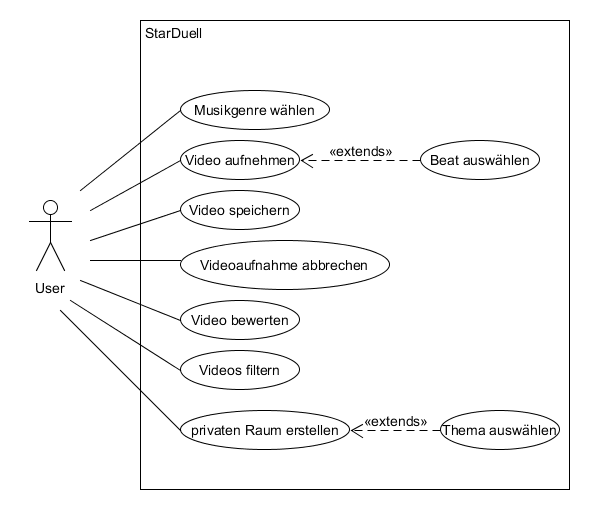
\includegraphics[width=0.7\linewidth]{images/UseCaseDiagramm}
			\caption{UseCase Diagramm}
			\label{fig:Usecase Diagramm}
		\end{figure}
		
		
	\section{\Large PRODUKTFUNKTIONEN}
	\subsection{Usecase-Beschreibungen}
	\begin{table}[H]
		\begin{tabular}{|p{8cm}|p{8cm}|}
			\hline
			\textbf{UC-01 } \\ 
			\hline
			\textbf{ID :}\centering & UC-01  \\ \hline 
			\textbf{Title :}\centering & Video aufnehmen \\ \hline 
			\textbf{Description :}\centering & Der User startet eine Videoaufnahme \\ \hline 
			\textbf{Trigger :}\centering & User tippt auf den "play" - Button \\ \hline 
			\textbf{Primary Actor :} \centering & User \\ \hline 
			\textbf{Preconditions :}\centering & 
				\\ \hline 
			\textbf{Postconditions :}\centering &  
			 \\ \hline
			\textbf{Other Use Cases :}\centering & - \\ \hline  
			\textbf{Main Success Scenario :}\centering & 
			 \\ \hline  
			\textbf{Extensions :}\centering & \\ \hline  
			\textbf{Priority :}\centering & High \\ \hline  
		\end{tabular}
	\end{table}	
	
	\begin{table}[H]
		\begin{tabular}{|p{8cm}|p{8cm}|}
			\hline
			\textbf{UC-02 } \\ 
			\hline
			\textbf{ID :}\centering & UC-02  \\ \hline 
			\textbf{Title :}\centering & Video speichern \\ \hline 
			\textbf{Description :}\centering & User speichert das Video in der Datenbank \\ \hline 
			\textbf{Trigger :}\centering & User tippt auf den Button "Speichern" \\ \hline 
			\textbf{Primary Actor :} \centering & User \\ \hline 
			\textbf{Preconditions :}\centering & 
			\\ \hline 
			\textbf{Postconditions :}\centering & 
			 \\ \hline
			\textbf{Other Use Cases :}\centering & - \\ \hline  
			\textbf{Main Success Scenario :}\centering & 
			\\ \hline  
			\textbf{Extensions :}\centering &  \\ \hline  
			\textbf{Priority :}\centering & High \\ \hline  
		\end{tabular}
	\end{table}
	
	\begin{table}[H]
		\begin{tabular}{|p{8cm}|p{8cm}|}
			\hline
			\textbf{UC-03 } \\ 
			\hline
			\textbf{ID :}\centering & UC-03  \\ \hline 
			\textbf{Title :}\centering & Videoaufnahme abbrechen  \\ \hline 
			\textbf{Description :}\centering & Der User bricht die Videoaufnahme ab und die bisherige Aufzeichnung wird verworfen  \\ \hline 
			\textbf{Trigger :}\centering & User tippt auf Button  \\ \hline 
			\textbf{Primary Actor :} \centering & User \\ \hline 
			\textbf{Preconditions :}\centering & 
			\\ \hline 
			\textbf{Postconditions :}\centering & 
			\\ \hline
			\textbf{Other Use Cases :}\centering & - \\ \hline  
			\textbf{Main Success Scenario :}\centering & 
			 \\ \hline  
			\textbf{Extensions :}\centering &  \\ \hline  
			\textbf{Priority :}\centering & High \\ \hline  
		\end{tabular}
	\end{table}
	
	\begin{table}[H]
		\begin{tabular}{|p{8cm}|p{8cm}|}
			\hline
			\textbf{UC-04 } \\ 
			\hline
			\textbf{ID :}\centering & UC-04  \\ \hline 
			\textbf{Title :}\centering & Video bewerten \\ \hline 
			\textbf{Description :}\centering & Ein User kann ein Video bewerten \\ \hline 
			\textbf{Trigger :}\centering & User tippt auf "Stern" - Button  \\ \hline 
			\textbf{Primary Actor :} \centering & User \\ \hline 
			\textbf{Preconditions :}\centering & 
			\\ \hline 
			\textbf{Postconditions :}\centering & 
			\\ \hline
			\textbf{Other Use Cases :}\centering & - \\ \hline  
			\textbf{Main Success Scenario :}\centering & 
			\\ \hline  
			\textbf{Extensions :}\centering & 
			\\ \hline  
			\textbf{Priority :}\centering & High \\ \hline  
		\end{tabular}
	\end{table}
	
	\begin{table}[H]
		\begin{tabular}{|p{8cm}|p{8cm}|}
			\hline
			\textbf{UC-05 } \\ 
			\hline
			\textbf{ID :}\centering & UC-05  \\ \hline 
			\textbf{Title :}\centering & Video filtern \\ \hline 
			\textbf{Description :}\centering & Dem User werden die Videos nach einem bestimmten Filter aufgelistet \\ \hline 
			\textbf{Trigger :}\centering & User bestimmt Filter und tippt auf Button \\ \hline 
			\textbf{Primary Actor :} \centering & User \\ \hline 
			\textbf{Preconditions :}\centering & 
			\\ \hline 
			\textbf{Postconditions :}\centering &
			\\ \hline
			\textbf{Other Use Cases :}\centering & - \\ \hline  
			\textbf{Main Success Scenario :}\centering &
			\\ \hline  
			\textbf{Extensions :}\centering &  \\ \hline  
			\textbf{Priority :}\centering & High \\ \hline  
		\end{tabular}
	\end{table}	
	
	\begin{table}[H]
		\begin{tabular}{|p{8cm}|p{8cm}|}
			\hline
			\textbf{UC-06 } \\ 
			\hline
			\textbf{ID :}\centering & UC-06  \\ \hline 
			\textbf{Title :}\centering & Musikgenre wählen \\ \hline 
			\textbf{Description :}\centering & Der User bestimmt das Musikgenre seines Videos \\ \hline 
			\textbf{Trigger :}\centering & User wählt aus einer Liste das Genre und bestätigt es mit einem Button \\ \hline 
			\textbf{Primary Actor :} \centering & User \\ \hline 
			\textbf{Preconditions :}\centering &\\ \hline 
			\textbf{Postconditions :}\centering	& 
			\\ \hline		
			\textbf{Other Use Cases :}\centering & - \\ \hline  
			\textbf{Main Success Scenario :}\centering &
			\\ \hline  
			\textbf{Extensions :}\centering & - \\ \hline  
			\textbf{Priority :}\centering & High \\ \hline  
		\end{tabular}
	\end{table}

	\begin{table}[H]
		\begin{tabular}{|p{8cm}|p{8cm}|}
			\hline
			\textbf{UC-07 } \\ 
			\hline
			\textbf{ID :}\centering & UC-07  \\ \hline 
			\textbf{Title :}\centering & privaten Raum erstellen \\ \hline 
			\textbf{Description :}\centering &  \\ \hline 
			\textbf{Trigger :}\centering & User klickt auf den Button "'Speichern Unter"' \\ \hline 
			\textbf{Primary Actor :} \centering & User \\ \hline 
			\textbf{Preconditions :}\centering & \\ \hline 
			\textbf{Postconditions :}\centering	& 
			\\ \hline		
			\textbf{Other Use Cases :}\centering & - \\ \hline  
			\textbf{Main Success Scenario :}\centering &
			\\ \hline  
			\textbf{Extensions :}\centering & \\ \hline  
			\textbf{Priority :}\centering & High \\ \hline  
		\end{tabular}
	\end{table}			
	
	\subsection{Aktivitätsdiagramm}

	\subsection{Sequenzdiagramm}
	
	
\newpage
	\section{\Large PRODUKTDATEN}
	
	\subsection{Analyseklassendiagramm}	
	
	\subsection{Paketdiagramm}
	
	\subsection{Domänenklassendiagramm}
	
	\section{\Large PRODUKTLEISTUNGEN}
	
	\section{\Large QUALITÄTSANFORDERUNGEN}
	
	
	\section{\Large BENUTZEROBERFLÄCHE}
	
	\subsection{Zustandsdiagramme}
	
	\section{\Large NICHTFUNKTIONALE ANFORDERUNGEN}
	

	
	\section{\Large TECHNISCHE PRODUKTUMGEBUNG}
   	In diesem Kapitel wird die technische Umgebung des Produkts beschrieben.\\
   	Bei Client / Server-Anwendungen ist die Umgebung jeweils für Clients und Server getrennt anzugeben.
	\subsection{Software}
	
	\subsection{Hardware}
	
	\subsection{Orgware}
	
	\subsection{Produkt-Schnittstellen}

	
	\section{\Large SPEZIELLE ANFORDERUNGEN AN DIE ENTWICKLUNGS-UMGEBUNG}
	
	\subsection{Software}
	\subsection{Hardware}
	\subsection{Orgware}
	\subsection{Entwicklungsschnittstellen}
	
	
	\section{\Large GLIEDERUNG IN TEILPRODUKTE}
	
	
	\section{\Large ERGÄNZUNGEN}
	.
	
\newpage
	\section{\Large GLOSSAR}
	In diesem Kapitel wird die spezifische Sprache des Auftraggebers wie \textbf{ Kürzel } und \textbf{ Fachbegriffe } beschrieben, z.B. :
	
		
		

\end{document}
%% Dokument ENDE %%%%%%%%%%%%%%%%%%%%%%%%%%%%%%%%%%%%%%%%%%%%%%%%%%%%%%%%%%

\grid
